\section{Ruta 2: Universidad de Ghana}

La ruta parte de Buenoa Aires, que es consistente ya que los paquetes fueron enviados desde ahi. Luego de no obtener respuesta en varios saltos, la siguiente respuesta sigue en Buenos Aires.
La ruta sigue en Estados Unidos, es posible que se utilice esta ruta a pesar de haber una mas corta (según el mapa de cables subacuáticos) porque al ser mas utilizadas las comunicaciones entre Argentina y America del Norte (particularmente Estados Unidos) que con África, es posible que los paquetes vayan mas rápido por esa ruta.
Luego hace un salto a Londres, que sería el segundo salto intercontinental. Siguiente, hace un salto a Singapur, que podría pensarse que se trata de un error de geolocalización. Sin embargo, el RTT es consistente con un envio por una ruta muy larga.
Luego los paquetes realizan varios saltos en Ghana hasta llegar a destino. 
Los saltos Buenos Aires-Ashburn, Ashburn-Londres y Singapur-Ghana son detectados correctamente. A la vez, hay muchos falsos positivos, en el caso del salto Londres-Singapur es entendible porque es un salto con un RTT muy alto, en los otros casos, pensamos que poría deberse a la aparición de RTTs con diferencia negativa con el salto anterior, que hacen que la detección de Outliers sea peor.


Paquetes enviados a www.ug.edu.gh

\begin{figure}[H]
\centering
\begin{tabular}{l | l | l | l | c | c}
Hop & RTT & IP & Ubicación & Predicción de SI & ¿correcto?\\
\hline
1 & 0.0231 & 192.168.0.1 & Buenos Aires, Argentina & true & \xmark\\
2 & null & null & null & null\\
3 & null & null & null & null\\
4 & null & null & null & null\\
5 & null & null & null & null\\
6 & null & null & null & null\\
7 & 0.2930 & \texttt{200.89.165.130} & Buenos Aires, Argentina & true & \xmark\\
8 & 0.1588 & \texttt{200.89.165.222} & Buenos Aires, Argentina & true & \xmark\\
9 & 0.1693 & \texttt{185.70.203.32} & Buenos Aires, Argentina & true & \xmark\\
10 & 0.2927 & \texttt{195.22.199.185} & Ashburn, EEUU & true & \cmark\\
11 & 0.1995 & \texttt{216.6.87.202} & Ashburn, EEUU & true & \xmark\\
12 & 0.6590 & \texttt{216.6.87.105} & Londres, Inglaterra & true & \cmark\\
13 & 0.3755 & \texttt{80.231.130.130} & Londres, Inglaterra & true & \xmark\\
14 & 0.4624 & \texttt{80.231.76.85} & Londres, Inglaterra & false & \cmark\\
15 & 1.0908 & \texttt{195.219.195.42} & Singapur, Singapur & true & \cmark\\
16 & 0.3648 & \texttt{41.204.60.149} & Kumasi, Ghana & true & \cmark\\
17 & 0.4641 & \texttt{41.204.60.150} & Kumasi, Ghana & false & \cmark\\
18 & 0.3928 & \texttt{197.255.127.6} & Accra, Ghana & true & \xmark\\
19 & 0.7883 & \texttt{197.255.127.35} & Accra, Ghana & true & \xmark\\
10 & 0.4128 & \texttt{197.255.125.213} & Accra, Ghana & true & \xmark\\
\end{tabular}
\caption{Tabla de resultados para la Universidad de Ghana.}
\label{tabla2}
\end{figure}

\begin{figure}[H]
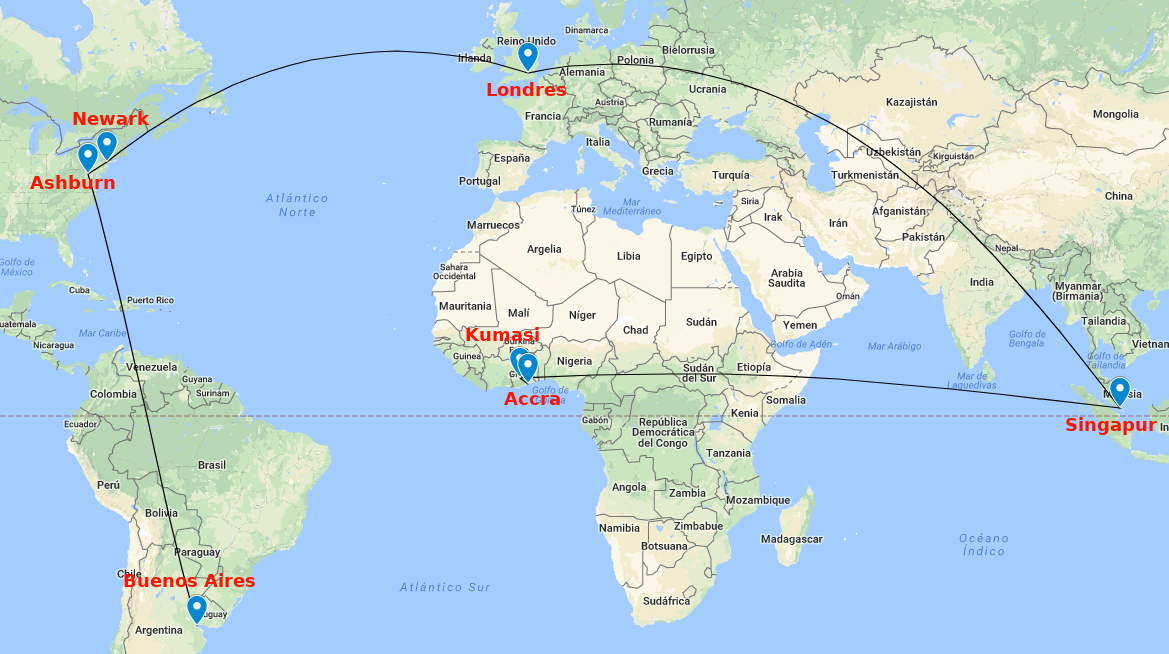
\includegraphics[width=\textwidth]{ghana.png}
\caption{Mapa de resultados para la Universidad de Ghana.}
\label{mapa2}
\end{figure}

\begin{figure}[H]
\centering
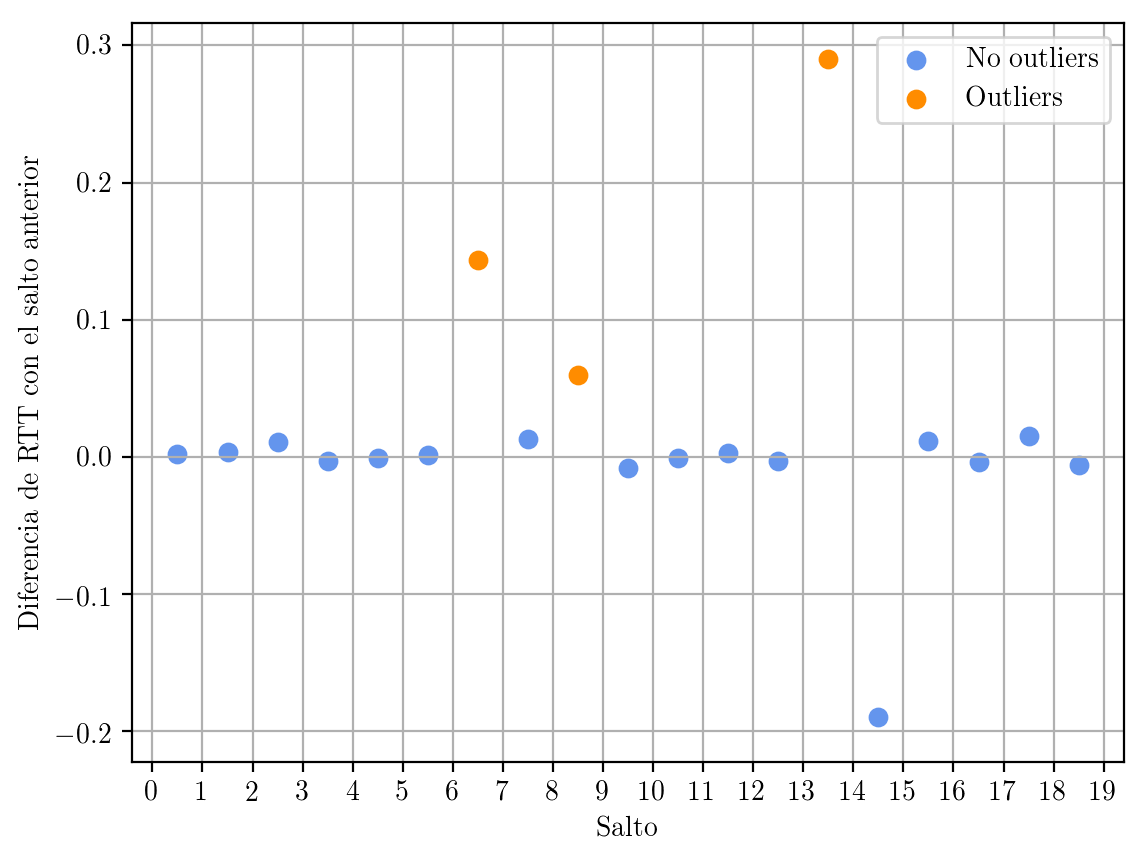
\includegraphics[width=0.6\textwidth]{ghana1.png}
\caption{Gráfico de diferencias de RTT en función de cada salto.}
\label{diff2}
\end{figure}

\begin{figure}[H]
\centering
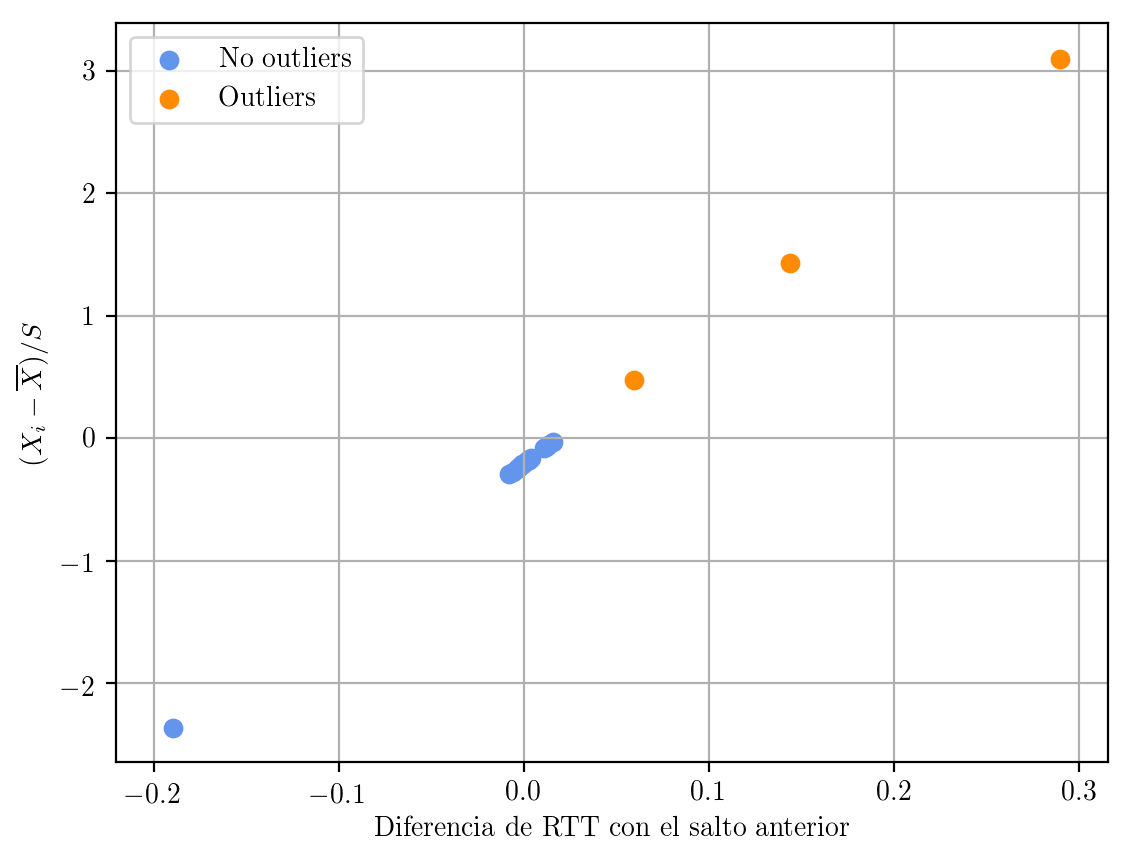
\includegraphics[width=0.6\textwidth]{ghana2.png}
\caption{Gráfico de $\frac{X_i - \bar{X}}{S}$ en función de las diferencias de RTT.}
\label{sdev2}
\end{figure}